\chapter{Entropy and the Second Law of Thermodynamics}\index{entropy}\index{second law of thermodynamics}

Your bedroom gets messy all by itself, but it never cleans itself. A mug of hot cocoa left on your
desk cools to room temperature; it never heats itself back up by pulling warmth out of the room. Drop
an egg and it splatters, but you will never see a splattered egg leap back into its shell.

None of these would break the law of conservation of energy. The cocoa could, in principle, take
heat from the room without creating or destroying any energy. Something else decides which way
things go. That something is \newterm{entropy}, and the rule it follows is the
\newterm{second law of thermodynamics}. The same rule tells you why no car engine can ever turn all of
its fuel into motion, and why a heat pump can heat a house so cheaply.

\section{The First Law, Briefly}\index{first law of thermodynamics}
You already know the first law: energy is never created or destroyed. For a gas in a cylinder, the
change in its internal energy $U$ (the kinetic energy of its molecules) is the heat $Q$ that flows in
minus the work $W$ the gas does on the outside world:
$$\Delta U = Q - W$$
The first law is an accounting rule. It tells you that the books must balance, but it says nothing
about which transactions actually happen. For that, we need the second law.

\section{Which Way Does Heat Flow?}
Put a hot pan in cool water, and heat flows from the pan to the water until they reach the same
temperature, as you saw in the Heat and Phases of Matter chapter. It never goes the other way on its own.

\begin{mdframed}[style = important, frametitle = {The Second Law (Heat Version)}]
Heat flows on its own from a hotter object to a colder one, never from colder to hotter.
\end{mdframed}

An air conditioner seems to break this rule: it moves heat from your cool house to the hot outdoors.
But it does not do it \emph{on its own}. It needs a compressor, plugged into the wall, doing work.
Unplug it, and the heat flows back in.

Why should heat care about direction? The answer comes from counting.

\section{Counting Microstates}\index{microstate}\index{macrostate}
Flip 4 coins. If you only care about how many came up heads, there are 5 possible results: 0, 1,
2, 3, or 4 heads. Each of these is a \newterm{macrostate}: a description of the big picture. But each
macrostate can happen in several ways. Each exact arrangement, like HTHT, is a
\newterm{microstate}. You learned to count them in the Counting chapter: the number of ways to get
$k$ heads from $n$ coins is $\binom{n}{k}$.

\begin{center}
\begin{tabular}{c|c|c}
Heads & Microstates & Count \\
\hline
0 & TTTT & 1 \\
1 & HTTT, THTT, TTHT, TTTH & 4 \\
2 & HHTT, HTHT, HTTH, THHT, THTH, TTHH & 6 \\
3 & THHH, HTHH, HHTH, HHHT & 4 \\
4 & HHHH & 1 \\
\end{tabular}
\end{center}

Every microstate is equally likely, so ``2 heads'' wins simply because it has the most ways to
happen.

Now flip 100 coins. There is exactly 1 way to get all heads. The number of ways to get 50 heads is
$$\binom{100}{50} \approx 1.01 \times 10^{29}$$
The half-and-half macrostate is not just more likely; it overwhelms everything else.

Gas molecules work the same way. Imagine a box with a wall down the middle and 100 molecules
crowded into the left half. Pull out the wall. Each molecule is equally likely to be on either side,
so the chance that all 100 are on the left at any moment is
$$\left(\tfrac{1}{2}\right)^{100} \approx 7.9 \times 10^{-31}$$
A real room holds about $10^{27}$ molecules, so the chance that all the air in your classroom
crowds into one corner is too small to write down. Nothing forbids it; it just never happens.

\subsection{Watching It Happen}
Here is a simple model of the box. At each step, pick a random molecule and move it to the other
side. Create a file called \filename{two\_rooms.py}:

\begin{minted}{python}
import random
import matplotlib.pyplot as plt

plt.rcParams["font.size"] = 14
random.seed(1)
n = 100                      # number of molecules
left = [True] * n            # every molecule starts on the left
counts = [n]

for step in range(1000):
    i = random.randrange(n)  # pick a random molecule...
    left[i] = not left[i]    # ...and move it to the other side
    counts.append(sum(left))

print("after 1000 steps:", counts[-1], "on the left")
print("average of the last 500 steps:", sum(counts[500:]) / len(counts[500:]))
print("all on the left again?", n in counts[1:])

plt.plot(counts)
plt.axhline(n / 2, color="gray", linestyle="--")
plt.xlabel("step")
plt.ylabel("molecules on the left")
plt.ylim(0, n)
plt.tight_layout()
plt.savefig("two_rooms.png", dpi=150)
\end{minted}

When you run it, you should see:
\begin{verbatim}
after 1000 steps: 56 on the left
average of the last 500 steps: 50.45109780439122
all on the left again? False
\end{verbatim}

\begin{figure}[!ht]
\centering
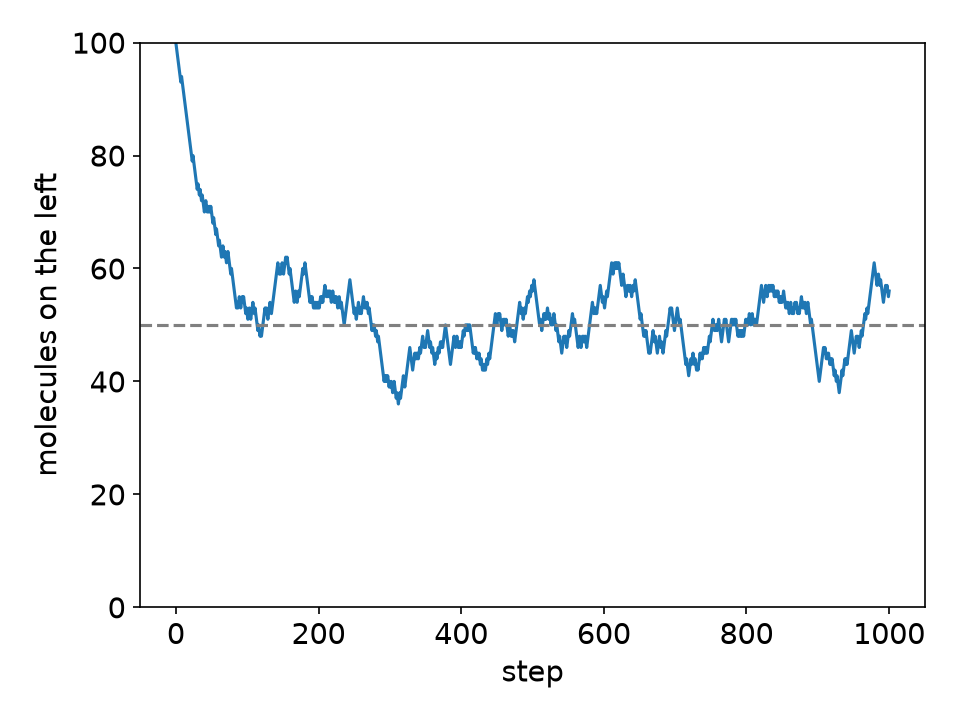
\includegraphics[width=0.7\textwidth]{two_rooms.png}
\caption{The molecules spread out until about half are on each side, then jiggle around 50 forever.}
\label{fig:two-rooms}
\end{figure}

No rule in the program pushes molecules to the right. Each move is completely random. The gas
spreads out only because there are vastly more half-and-half arrangements than lopsided ones. That
is the second law: systems drift toward the macrostates with the most microstates.

\subsection{Entropy Is Counting}\index{Boltzmann's entropy formula}
Ludwig Boltzmann turned this idea into a formula. If a macrostate can happen in $W$ ways, its entropy is
\begin{mdframed}[style = important, nobreak = true, frametitle = {Boltzmann's Entropy}]
$$S = k \ln W$$
where $k = 1.38 \times 10^{-23}$ J/K is Boltzmann's constant.
\end{mdframed}
Boltzmann thought this formula was so important that it is carved on his tombstone.

Why the logarithm? Put two systems side by side. If one can be arranged in $W_1$ ways and the other in
$W_2$ ways, together they can be arranged in $W_1 W_2$ ways. The logarithm turns that product into a
sum, $\ln(W_1W_2) = \ln W_1 + \ln W_2$, so entropies add, just as masses and energies do.

\begin{mdframed}[style = important, frametitle = {The Second Law (Entropy Version)}]
The total entropy of an isolated system never decreases.
\end{mdframed}

\section{Entropy and Heat}\index{entropy!and heat}
Counting microstates of $10^{27}$ molecules is hopeless, but there is a shortcut. When a small amount
of heat $Q$ flows into an object at temperature $T$ (in kelvins), its entropy changes by
$$\Delta S = \frac{Q}{T}$$
Adding heat gives molecules more ways to share energy, so entropy rises. The same heat matters more
to a cold object than to a hot one, which is why $T$ is in the denominator.

\textbf{Example}: Your cocoa is at 350 K and your room is at 300 K. Suppose 1,000 J of heat flows from
the cocoa to the room. (Both temperatures barely change during this small flow.) What happens to the
total entropy?

\textbf{Solution}: The cocoa loses heat, so its entropy falls:
$$\Delta S_{\text{cocoa}} = \frac{-1000}{350} \approx -2.86 \text{ J/K}$$
The room gains the same heat at a lower temperature, so its entropy rises by more:
$$\Delta S_{\text{room}} = \frac{1000}{300} \approx 3.33 \text{ J/K}$$
The total rises by about $0.48$ J/K. If the heat flowed the other way, from the room into the cocoa,
every sign would flip and the total would \emph{fall}. That is forbidden, so cocoa never heats itself
up. The heat version and the entropy version of the second law are the same law.

\textbf{Example}: In the Heat and Phases of Matter chapter, you learned that melting ice takes 6.01 kJ per
mole, which is about 334 J per gram. What is the entropy change when 10 g of ice melts at 273 K?

\textbf{Solution}: $Q = (10)(334) = 3340$ J, all absorbed at 273 K, so
$$\Delta S = \frac{3340}{273} \approx 12.2 \text{ J/K}$$
Liquid water has more entropy than ice: the molecules are no longer locked in a crystal, so there are
far more ways to arrange them.

\section{Heat Engines and the Carnot Limit}\index{heat engine}\index{Carnot efficiency}
In the Piston Engine chapter, you learned that a car engine turns only about 30\% of its fuel's energy into
turning the crankshaft. Better engineering helps, but no engine, however perfect, can reach 100\%.
Entropy explains why.

Every \newterm{heat engine} works the same way. It takes in heat $Q_H$ from something hot (burning fuel,
steam), turns part of it into work $W$, and dumps the rest, $Q_C$, into something cold (the air, a river).

\begin{figure}[htbp]
\centering
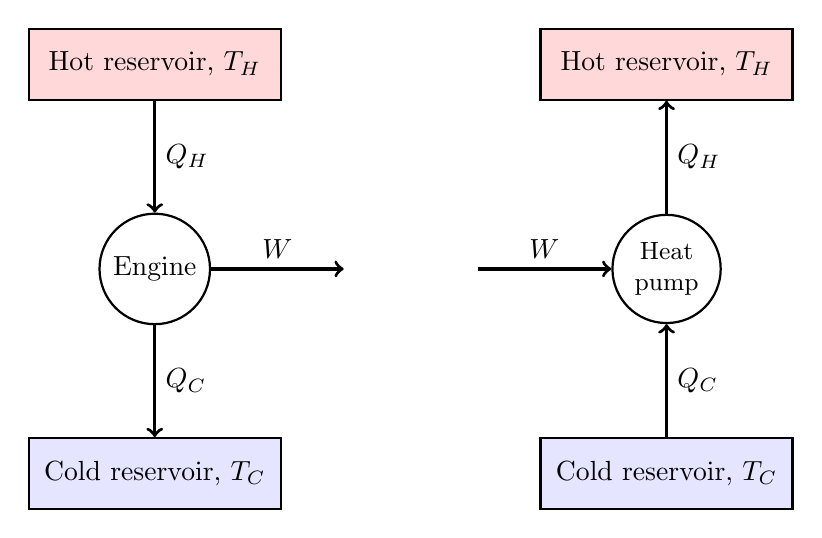
\begin{tikzpicture}[box/.style={draw, thick, minimum width=3.2cm, minimum height=0.9cm, align=center}]
  \node[box, fill=red!15] (hot) at (0,2.6) {Hot reservoir, $T_H$};
  \node[draw, thick, circle, minimum size=1.3cm] (eng) at (0,0) {Engine};
  \node[box, fill=blue!10] (cold) at (0,-2.6) {Cold reservoir, $T_C$};
  \draw[->, very thick] (hot) -- node[right] {$Q_H$} (eng);
  \draw[->, very thick] (eng) -- node[right] {$Q_C$} (cold);
  \draw[->, very thick] (eng) -- node[above] {$W$} (2.4,0);

  \node[box, fill=red!15] (hot2) at (6.5,2.6) {Hot reservoir, $T_H$};
  \node[draw, thick, circle, minimum size=1.3cm, align=center, font=\small] (fr) at (6.5,0) {Heat\\pump};
  \node[box, fill=blue!10] (cold2) at (6.5,-2.6) {Cold reservoir, $T_C$};
  \draw[->, very thick] (fr) -- node[right] {$Q_H$} (hot2);
  \draw[->, very thick] (cold2) -- node[right] {$Q_C$} (fr);
  \draw[->, very thick] (4.1,0) -- node[above] {$W$} (fr);
\end{tikzpicture}
\caption{Left: a heat engine turns part of the heat flowing from hot to cold into work. Right: a refrigerator or heat pump uses work to push heat from cold to hot.}
\label{fig:engine-diagram}
\end{figure}

The \newterm{efficiency} is the fraction of the heat that becomes work:
$$e = \frac{W}{Q_H} = \frac{Q_H - Q_C}{Q_H}$$

Now track the entropy. The hot reservoir loses $Q_H/T_H$ of entropy. The cold reservoir gains $Q_C/T_C$.
The engine itself returns to the same state after every cycle, so its entropy does not change. Work
carries no entropy. The second law says the total cannot fall:
$$\frac{Q_C}{T_C} \geq \frac{Q_H}{T_H} \qquad\text{so}\qquad \frac{Q_C}{Q_H} \geq \frac{T_C}{T_H}$$
The engine \emph{must} dump some heat into the cold reservoir, or the entropy would go down. Substitute
into the efficiency:

\begin{mdframed}[style = important, frametitle = {The Carnot Limit}]
$$e \leq 1 - \frac{T_C}{T_H}$$
Temperatures must be in kelvins.
\end{mdframed}

Sadi Carnot, a French engineer, found this limit in 1824 by thinking about steam engines, decades
before anyone understood entropy. An engine that reaches the limit exactly is called a
\newterm{Carnot engine}. It would have to run infinitely slowly, so real engines always fall short.

\textbf{Example}: A power plant heats steam to 800 K and cools it with river water at 300 K. What is
the best possible efficiency?

\textbf{Solution}:
$$e \leq 1 - \frac{300}{800} = 0.625$$
At most 62.5\%. Real plants like this one reach about 40\%. If this plant sends 1,000 MW of electricity
to the grid at 40\% efficiency, it burns fuel at $1000/0.4 = 2{,}500$ MW and dumps $1{,}500$ MW of heat
into the river and air. That is what those giant cooling towers are for.

The Carnot limit explains a lesson from the Piston Engine chapter: a higher compression ratio makes the burning
gas hotter, which raises $T_H$, which raises the limit. To make any engine more efficient, make the hot
side hotter or the cold side colder.

\section{Refrigerators and Heat Pumps}\index{heat pump}\index{coefficient of performance}
Run an engine backwards and you get a refrigerator: work $W$ pulls heat $Q_C$ out of the cold inside and
dumps $Q_H = Q_C + W$ into your warm kitchen. The coils on the back of your fridge are warm because
they are getting rid of that heat.

For a heat pump warming a house in winter, what you want is the heat delivered inside, $Q_H$. Its
\newterm{coefficient of performance} is
$$\text{COP} = \frac{Q_H}{W}$$
The same entropy argument (try it in an exercise) gives the limit
$$\text{COP} \leq \frac{T_H}{T_H - T_C}$$

\textbf{Example}: It is 0\textdegree C (273 K) outside, and you want to keep your house at 20\textdegree C
(293 K). What is the best possible COP?

\textbf{Solution}:
$$\text{COP} \leq \frac{293}{293 - 273} = \frac{293}{20} \approx 14.7$$
A perfect heat pump would deliver almost 15 joules of heat for each joule of electricity. Real ones
deliver about 3. Even so, that beats an electric space heater, which turns each joule of electricity into
exactly 1 joule of heat. A heat pump does not make heat; it moves heat that is already outside, and
moving heat is cheaper than making it.

Notice that the COP gets worse as the outside gets colder: the bigger $T_H - T_C$ is, the harder the pump
must work.

\section{Order Without Breaking the Law}
If entropy always increases, how can a snowflake form, a seed grow into a tree, or you clean your room?
Each of these makes something more orderly, which lowers its entropy.

The answer is the word \emph{isolated}. A snowflake freezes by releasing heat into the cold air, and
that heat raises the air's entropy by more than the snowflake loses. A tree uses sunlight. You burn
breakfast to clean your room, and give off heat as you do it. Order can grow in one place, as long as
more disorder is pushed somewhere else.

The second law also tells time which way to run. Almost every other law of physics works just as well
backwards: a video of two billiard balls colliding looks fine played in reverse. A video of an egg unbreaking does not. The
direction we call ``the future'' is the direction in which entropy increases. Followed to the end, it
leads to the heat death of the universe, which the chapter on matter and energy mentioned: everything
at one temperature, with no flow of heat left to run anything.

\begin{Exercise}[title={Six Coins}, label=sl_coins]
You flip 6 coins. How many microstates have exactly 3 heads? What is the probability of getting exactly
3 heads? What is the probability of getting all heads?
\end{Exercise}
\begin{Answer}[ref=sl_coins]
$\binom{6}{3} = 20$ microstates have 3 heads. There are $2^6 = 64$ microstates in all, so the probability
is $20/64 \approx 0.31$. All heads is 1 microstate, so its probability is $1/64 \approx 0.016$.
\end{Answer}

\begin{Exercise}[title={Ice in Your Drink}, label=sl_ice]
You drop 20 g of ice at 273 K into a drink at 293 K. Assume all of the ice melts, absorbing 334 J/g,
and that the drink stays near 293 K. Find the entropy change of the ice, of the drink, and of the two
together.
\end{Exercise}
\begin{Answer}[ref=sl_ice]
$Q = (20)(334) = 6680$ J. The ice gains $6680/273 \approx 24.5$ J/K. The drink loses
$6680/293 \approx 22.8$ J/K. The total increases by about $1.7$ J/K, as the second law requires.
\end{Answer}

\begin{Exercise}[title={An Inventor's Claim}, label=sl_claim]
An inventor says their new engine runs between a hot reservoir at 400 K and a cold one at 300 K, with
an efficiency of 30\%. Should you invest?
\end{Exercise}
\begin{Answer}[ref=sl_claim]
No. The Carnot limit is $1 - 300/400 = 0.25$, or 25\%. No engine working between these temperatures
can reach 30\%.
\end{Answer}

\begin{Exercise}[title={Geothermal Power}, label=sl_geo]
A geothermal plant uses underground water at 450 K and cools it with air at 300 K. What is its maximum
efficiency? Why do geothermal plants have lower efficiencies than plants that burn fuel?
\end{Exercise}
\begin{Answer}[ref=sl_geo]
$e \leq 1 - 300/450 \approx 0.33$, or 33\%. Underground water is much cooler than burning fuel or steam
from a boiler, so $T_H$ is low and the Carnot limit is low.
\end{Answer}

\begin{Exercise}[title={A Cold Snap}, label=sl_cold]
The outside temperature drops to $-10$\textdegree C (263 K), and the house is still kept at 293 K.
Find the best possible COP of the heat pump, and compare it with the 0\textdegree C example.
\end{Exercise}
\begin{Answer}[ref=sl_cold]
$\text{COP} \leq 293/(293-263) = 293/30 \approx 9.8$, down from about 14.7. The colder it gets outside, the
more work each joule of heat costs. This is why some homes keep a backup heater for the coldest days.
\end{Answer}

\begin{Exercise}[title={Open the Fridge}, label=sl_fridge]
On a hot day, could you cool your kitchen by leaving the refrigerator door open?
\end{Exercise}
\begin{Answer}[ref=sl_fridge]
No. The fridge pulls heat $Q_C$ from the air in front of it and dumps $Q_H = Q_C + W$ out the back, into
the same kitchen. The kitchen gains a net $W$, the electrical energy the fridge uses, so it gets
\emph{warmer}. An air conditioner works only because it dumps $Q_H$ outside.
\end{Answer}

\begin{Exercise}[title={Proving the Heat Pump Limit}, label=sl_cop]
Use the entropy argument from the Carnot section to prove that a heat pump's COP is at most
$T_H/(T_H - T_C)$. (Hint: now the cold reservoir loses $Q_C/T_C$ and the hot reservoir gains $Q_H/T_H$,
with $Q_C = Q_H - W$.)
\end{Exercise}
\begin{Answer}[ref=sl_cop]
The total entropy cannot fall, so $Q_H/T_H \geq Q_C/T_C = (Q_H - W)/T_C$. Multiply by $T_H T_C$:
$Q_H T_C \geq (Q_H - W) T_H$, so $W T_H \geq Q_H (T_H - T_C)$. Dividing,
$$\text{COP} = \frac{Q_H}{W} \leq \frac{T_H}{T_H - T_C}$$
\end{Answer}

\begin{Exercise}[title={More Molecules}, label=sl_more]
Make your simulation in \filename{two\_rooms.py} use 1,000 molecules and 10,000 steps. After the gas has spread out,
the count on the left wanders around 500. Is the wandering bigger or smaller, as a fraction of all the
molecules, than it was with 100?
\end{Exercise}
\begin{Answer}[ref=sl_more]
Smaller. With 100 molecules, the count typically strays about 5 from 50, which is 5\% of the molecules.
With 1,000, it strays about 16 from 500, only about 1.6\%. The typical wandering grows like $\sqrt{n}$,
so as a fraction it shrinks like $1/\sqrt{n}$. With $10^{27}$ molecules, the fluctuations are far too
small to ever notice, which is why the second law looks perfectly strict for everyday objects.
\end{Answer}
